\section{Digitalisierung von Signalen S. 79}
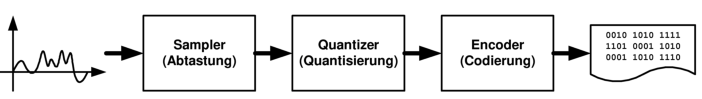
\includegraphics{chapters/07_digsig/figures/digitalisierungBlockschema.pdf}
\begin{table}[H]
	\begin{tabularx}{\linewidth}{X|X}
		\begin{list}{$\bullet$}{\setlength{\itemsep}{0cm} \setlength{\parsep}{0cm}
				\setlength{\topsep}{0cm}} 
				\item Zeitdiskretisierung, endliche Anzahl von Werten pro Zeit
				\item störungsfreie Übertragung
				\item Codierung (z.B. Fehlerkorrektur oder Verschlüsselung)
		\end{list}
	&
		\begin{list}{$\bullet$}{\setlength{\itemsep}{0cm} \setlength{\parsep}{0cm}
		\setlength{\topsep}{0cm}} 
			\item Quantisierung, endliche Anzahl an Amplitudenwerten (Bits)
			\item neue Möglichkeiten für Signalverarbeitung
			\item Speicherung auf einheitlichen Medien
	\end{list}
	\end{tabularx}
\end{table}

\subsection{Abtastung S. 80}
\subsubsection{Ideale Abtastung S.82}
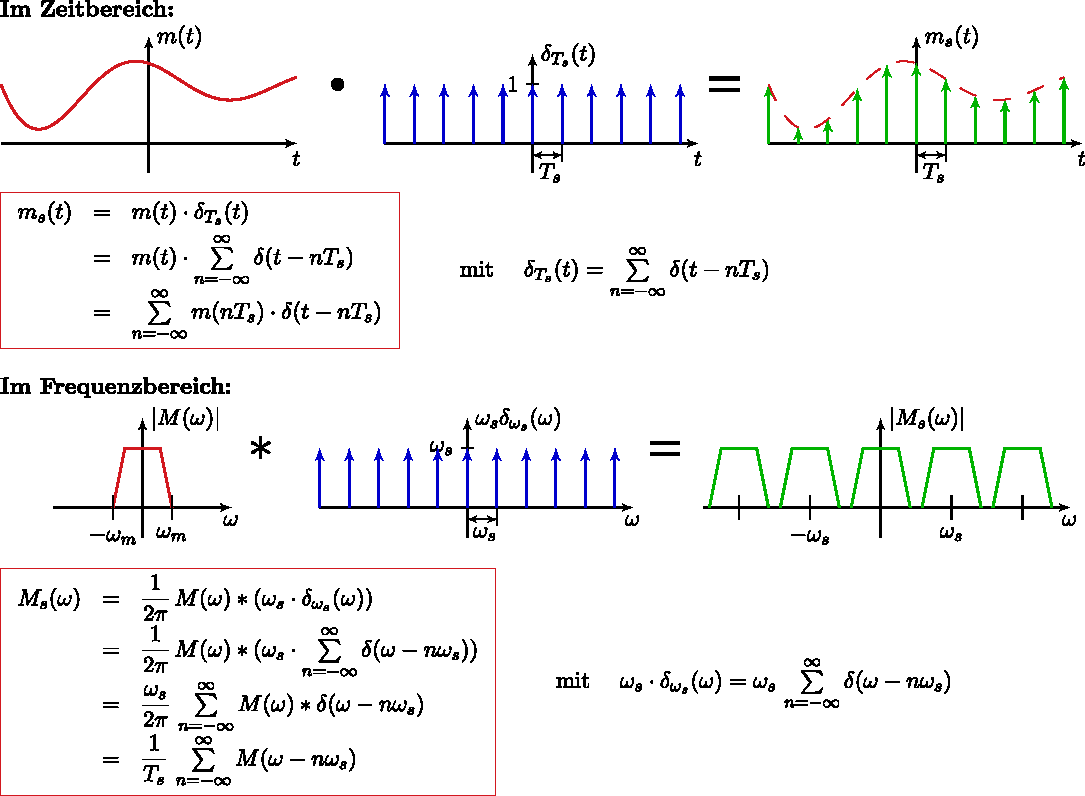
\includegraphics[width=.90\linewidth]{chapters/07_digsig/figures/idealeAbtastung.pdf}

\subsubsection{Rekonstruktion mit Tiefpass S. 87}
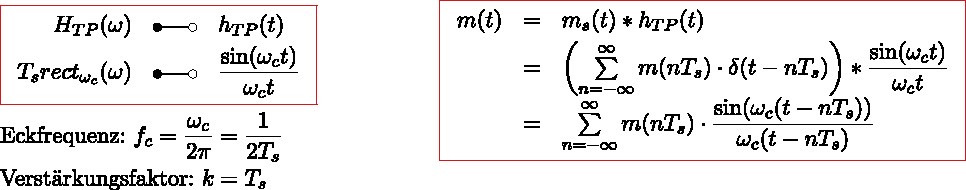
\includegraphics[width=.95\linewidth]{chapters/07_digsig/figures/rekonstruktionTP.pdf}

\subsubsection{Natural Sampling S. 81}
$m(t)$ wird mit einer Folge von Rechteckpulsen (Breite $\tau$, Periode $T_s$) multipliziert; innerhalb des Pulses folgt $m_{NS}$ dem Signal.\\[.3em]
\efbox[linecolor=red]{$m_{NS}(t) = m(t) \cdot \displaystyle\sum_{n=-\infty}^{\infty} \mathrm{rect}_{\tau/2}(t - nT_s)$}
\quad $\Rightarrow$ \quad
\efbox[linecolor=red]{$M_{NS}(\omega) = \displaystyle\sum_{n=-\infty}^{\infty} c_n \cdot M(\omega - n\omega_s)$}
\quad $c_n = \dfrac{\tau}{T_s} \cdot \dfrac{\sin\left(n\,\omega_s\,\tau/2\right)}{n\,\omega_s\,\tau/2}$, \qquad $c_0 = \dfrac{\tau}{T_s}$
\\[.4em]
\textrightarrow\ Kopien von $M$ bei $n\,\omega_s$, jede nur mit der Konstante $c_n$ skaliert: die \textbf{Form bleibt} $\Rightarrow$ unverzerrt\\
% Natural Sampling kompakt: Zeitbereich (links) <-> Frequenzbereich (rechts), Zeilen: m, p, m_NS (mit Tiefpass).
% tau/T_s = 0,4 : c_0 = 0,4 ; c_1 = 0,303 ; c_2 = 0,094. Frequenzachse in Einheiten von omega_s, omega_M = 0,32 omega_s.
\begin{center}
\resizebox{.95\linewidth}{!}{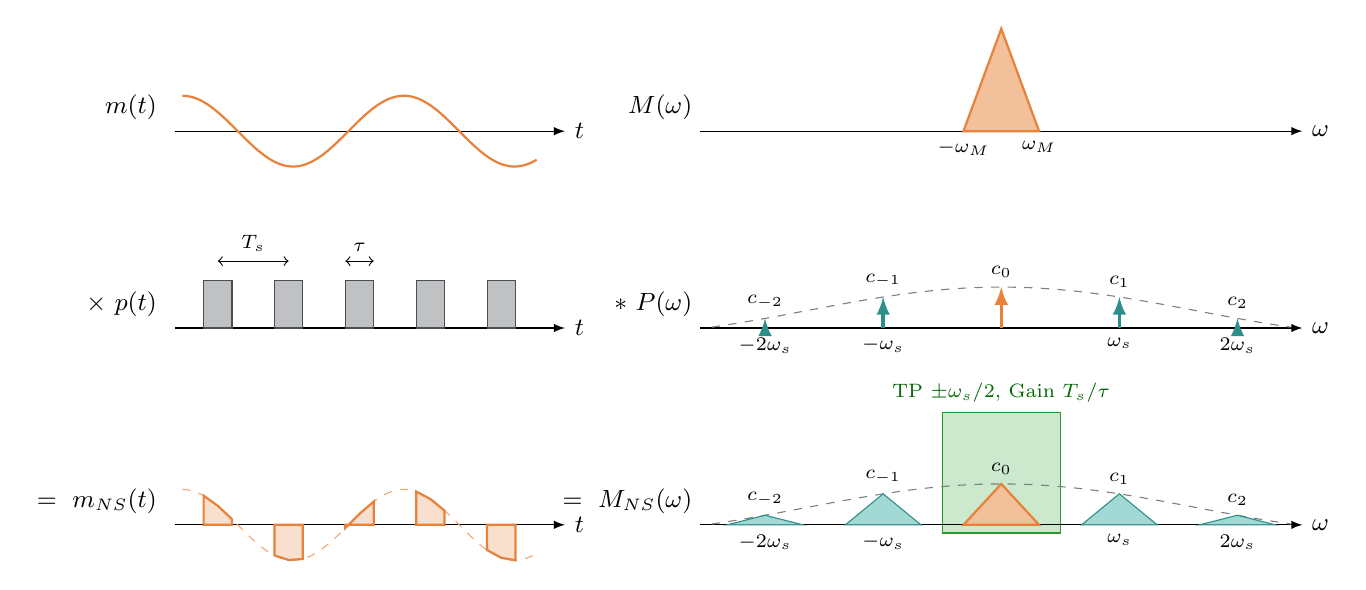
\begin{tikzpicture}[lab/.style={font=\small},tk/.style={font=\scriptsize},ax/.style={-latex,thin}]
\definecolor{org}{HTML}{E8813A}
\definecolor{kA}{HTML}{8CCFCB}\definecolor{kAd}{HTML}{2E8F8A}
\definecolor{ard}{HTML}{4A4D52}
\definecolor{flt}{HTML}{BFE3C0}
\def\pM{0.32}\def\dtau{0.4}
\node[lab,anchor=east] at (1.5,0.3) {$m(t)$};              \node[lab,anchor=east] at (8.3,0.3) {$M(\omega)$};
\node[lab,anchor=east] at (1.5,-2.2) {$\times\ p(t)$};     \node[lab,anchor=east] at (8.3,-2.2) {$\ast\ P(\omega)$};
\node[lab,anchor=east] at (1.5,-4.7) {$=\ m_{NS}(t)$};     \node[lab,anchor=east] at (8.3,-4.7) {$=\ M_{NS}(\omega)$};
% ---------- Zeitbereich ----------
\begin{scope}[shift={(1.7,0)},x=0.9cm,y=1cm]
  \draw[ax] (-0.1,0) -- (5.4,0) node[right,lab] {$t$};
  \draw[org,thick,domain=0:5,samples=50,smooth] plot (\x,{0.45*cos(360*\pM*\x)});
\end{scope}
\begin{scope}[shift={(1.7,-2.5)},x=0.9cm,y=1cm]
  \draw[ax] (-0.1,0) -- (5.4,0) node[right,lab] {$t$};
  \foreach \c in {0.5,1.5,2.5,3.5,4.5} \fill[ard!35,draw=ard] (\c-0.2,0) rectangle (\c+0.2,0.6);
  \draw[<->] (0.5,0.85) -- (1.5,0.85) node[midway,above,tk] {$T_s$};
  \draw[<->] (2.3,0.85) -- (2.7,0.85) node[midway,above,tk] {$\tau$};
\end{scope}
\begin{scope}[shift={(1.7,-5)},x=0.9cm,y=1cm]
  \draw[ax] (-0.1,0) -- (5.4,0) node[right,lab] {$t$};
  \draw[org!70,dashed,domain=0:5,samples=50,smooth] plot (\x,{0.45*cos(360*\pM*\x)});
  \foreach \c in {0.5,1.5,2.5,3.5,4.5}
    \filldraw[fill=org!25,draw=org,thick] (\c-0.2,0) -- plot[domain=\c-0.2:\c+0.2,samples=3] (\x,{0.45*cos(360*\pM*\x)}) -- (\c+0.2,0) -- cycle;
\end{scope}
% ---------- Frequenzbereich (Einheit omega_s, Höhe 1 = Spitze von M) ----------
\begin{scope}[shift={(12.1,0)},x=1.5cm,y=1.3cm]
  \draw[ax] (-2.55,0) -- (2.55,0) node[right,lab] {$\omega$};
  \fill[org!50,draw=org,thick] (-\pM,0) -- (0,1) -- (\pM,0) -- cycle;
  \node[tk,below] at (-\pM,0) {$-\omega_M$}; \node[tk,below] at (\pM,0) {$\omega_M$};
\end{scope}
\begin{scope}[shift={(12.1,-2.5)},x=1.5cm,y=1.3cm]
  \draw[ax] (-2.55,0) -- (2.55,0) node[right,lab] {$\omega$};
  \draw[dashed,gray,domain=-2.45:2.45,samples=50] plot (\x,{\dtau*sin(deg(pi*\dtau*\x))/(pi*\dtau*\x)});
  \foreach \n/\h/\l in {-2/0.094/c_{-2},-1/0.303/c_{-1},1/0.303/c_1,2/0.094/c_2}
    {\draw[-latex,very thick,kAd] (\n,0) -- (\n,\h); \node[tk,above] at (\n,\h) {$\l$};}
  \draw[-latex,very thick,org] (0,0) -- (0,0.4); \node[tk,above] at (0,0.4) {$c_0$};
  \foreach \n/\t in {-2/-2\omega_s,-1/-\omega_s,1/\omega_s,2/2\omega_s} \node[tk,below] at (\n,0) {$\t$};
\end{scope}
\begin{scope}[shift={(12.1,-5)},x=1.5cm,y=1.3cm]
  \fill[flt,opacity=0.8,draw=green!50!black,thin] (-0.5,-0.08) rectangle (0.5,1.1);
  \node[tk,above,text=green!40!black] at (0,1.1) {TP $\pm\omega_s/2$, Gain $T_s/\tau$};
  \draw[ax] (-2.55,0) -- (2.55,0) node[right,lab] {$\omega$};
  \draw[dashed,gray,domain=-2.45:2.45,samples=50] plot (\x,{\dtau*sin(deg(pi*\dtau*\x))/(pi*\dtau*\x)});
  \foreach \n/\h/\l in {-2/0.094/c_{-2},-1/0.303/c_{-1},1/0.303/c_1,2/0.094/c_2}
    {\fill[kA,fill opacity=0.8,draw=kAd] (\n-\pM,0) -- (\n,\h) -- (\n+\pM,0) -- cycle; \node[tk,above] at (\n,\h) {$\l$};}
  \fill[org!50,draw=org,thick] (-\pM,0) -- (0,0.4) -- (\pM,0) -- cycle; \node[tk,above] at (0,0.4) {$c_0$};
  \foreach \n/\t in {-2/-2\omega_s,-1/-\omega_s,1/\omega_s,2/2\omega_s} \node[tk,below] at (\n,0) {$\t$};
\end{scope}
\end{tikzpicture}}
\end{center}

\definecolor{ardesia}{HTML}{4A4D52}\definecolor{papier}{HTML}{F6F5F1}
\efbox[linecolor=ardesia,backgroundcolor=papier]{\begin{minipage}{.96\linewidth}
\textbf{Rekonstruktion}\\[.1em]
{\renewcommand{\arraystretch}{1.4}
\begin{tabularx}{\linewidth}{l X}
	1. & Tiefpass bis $\omega_s/2$ mit Verstärkung $\dfrac{T_s}{\tau} = \dfrac{1}{c_0}$ (hebt die Dämpfung $c_0$ wieder auf) \\
	2. & es passt nur die Kopie $n = 0$ \; $\Leftrightarrow$ \; $\omega_s > 2\,\omega_{max}$ \\
	3. & $m_r(t) = m(t)$ \\
\end{tabularx}}
\end{minipage}}\\[.3em]
{\small \textrightarrow\ ZOH: die $\mathrm{sinc}$ multipliziert das \textbf{ganze} Spektrum $\Rightarrow$ Verzerrung}\\
{\small \textrightarrow\ kleineres $\tau$: kleineres $c_0$, flachere Hüllkurve; $\tau \to 0$ ist die ideale Abtastung}

\subsubsection{Sample {\&} Hold (ZOH), Flat-Top Sampling S. 90}
ZOH $\rightarrow$ Zero Order Hold. $H_{ZOH}(\omega) = \tau \cdot \frac{sin(\frac{\tau \omega}{2})}{\frac{\tau \omega}{2 }} \;\;\; , \;\;\; \tau \leq T_s$\\
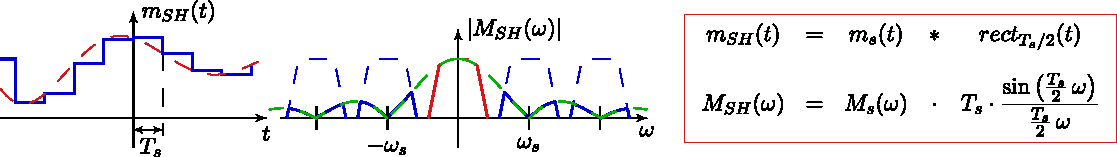
\includegraphics{chapters/07_digsig/figures/flattopsampling.pdf}

\paragraph{Rekonstruktion im Vergleich}
{\renewcommand{\arraystretch}{1.7}
\begin{tabularx}{\linewidth}{l l l X}
	\textbf{Methode} & \textbf{Impuls ersetzt $\delta(t - kT_s)$} & \textbf{Filter} & \textbf{$|H(f_s/2)|/|H(0)|$} \\ \hline
	sinc (ideal) & $\dfrac{\sin\left(\pi \frac{t-kT_s}{T_s}\right)}{\pi \frac{t-kT_s}{T_s}}$ & Rechteck bis $f_s/2$ & $1$ \\
	linear & $x_{tri}\left(\dfrac{t-kT_s}{2T_s}\right)$ & $T_s \cdot \left(\dfrac{\sin(\omega T_s/2)}{\omega T_s/2}\right)^2$ & $0.41$ ($-7.8$ dB) \\
	ZOH & $x_{rect}\left(\dfrac{t-kT_s}{\tau_p}\right)$ & $\tau_p \cdot \dfrac{\sin(\omega \tau_p/2)}{\omega \tau_p/2}$ & $0.64$ ($-3.9$ dB), bei $\tau_p = T_s$ \\
\end{tabularx}}\\
{\small \textrightarrow\ ZOH: Kopien bei $\pm n f_s$ nur gedämpft $\Rightarrow$ analoges Rekonstruktionsfilter nötig}\\
{\small \textrightarrow\ kürzere $\tau_p$: weniger Dämpfung im Basisband, Filter bleibt gleich anspruchsvoll}

\subsubsection{Nyquist-Shannon Abtasttheorem S. 85}
	\begin{list}{$\bullet$}{\setlength{\itemsep}{0cm} \setlength{\parsep}{0cm}
	\setlength{\topsep}{0cm}} 
		\item Nachrichtensignal muss auf eine Bandbreite begrenzt sein $|M(\omega)|\approx 0 \text{ für } \omega > 2\pi B_m$ (Aliasing S. 87)
		\item im Basisband darf es keine Überlappungen von Teilspektren geben, d.h. $f_s$ muss die Spektralanteile genügend weit vom ursprünglichen Spektrum wegschieben.
	\end{list}

\begin{minipage}{.3\linewidth}
	\textbf{Abtasttheorem für Basisbandsignale:} \efbox[linecolor=red]{$f_s > 2 \cdot B_m$}\\[.3em]
	{\small Einheiten: $[f_s] = [f_m] = [B_m] = \si{\hertz}$}
\end{minipage}
\begin{minipage}{.7\linewidth}
	{\renewcommand{\arraystretch}{1.6}
	\begin{tabularx}{\linewidth}{l l X}
		\textbf{Grösse} & \textbf{Formel} & \textbf{Bedeutung} \\ \hline
		Nyquist-Rate      & $f_s > f_{s_N} = 2 B_m$ & minimale Samplerate \\
		Nyquist-Frequenz  & $f_N = \dfrac{f_s}{2}$ & max. Frequenz bei gegebenem $f_s$ \\
		Nyquist-Intervall & $T_s < T_{s_N} = \dfrac{1}{2 B_m}$ & max. Abstand der Samples \\
		Nyquist-Zonen     & $0\ldots\tfrac{f_s}{2} \;|\; \tfrac{f_s}{2}\ldots f_s \;|\; \ldots$ & gerade Zonen: Spektrum gespiegelt \\
	\end{tabularx}}
\end{minipage}

\paragraph{Aliasing}
Antialiasing-TP \textbf{vor} dem A/D-Wandler (auch gegen Störsignale).\\
{\small \textrightarrow\ Alias-Frequenz: $f_a = |f - k \cdot f_s|$, $k$ = nächste ganze Zahl zu $f/f_s$}\\
{\small \textrightarrow\ nach der Abtastung nicht mehr vom Nutzsignal trennbar}

\paragraph{Abtasttheorem für Bandpasssignale S. 85 (Subsampling)}
Nach dem Sampling wiederholt sich das Spektrum bei jedem $k \cdot f_s$; Band $[f_l, f_u]$ \textbf{und} Spiegelband $[-f_u, -f_l]$ wandern mit. Die Kopien müssen in die Lücken passen, ein Basisband ist nicht nötig. \textbf{Nur möglich}, wenn das Band \textbf{nicht im Basisband} liegt ($f_l > 0$, es berührt nicht $f = 0$); sonst bleibt $f_s > 2 f_u$.\\[.2em]
% Subsampling: Kopien des Bandpass-Spektrums. Farbe = Verschiebung k*f_s (Tick auf der Achse = gleiche Farbe wie die zwei Rechtecke).
% Oben f_s im Fenster, unten ausserhalb. Einheiten beliebig: f_l=3, f_u=5.
\begin{center}
\resizebox{.92\linewidth}{!}{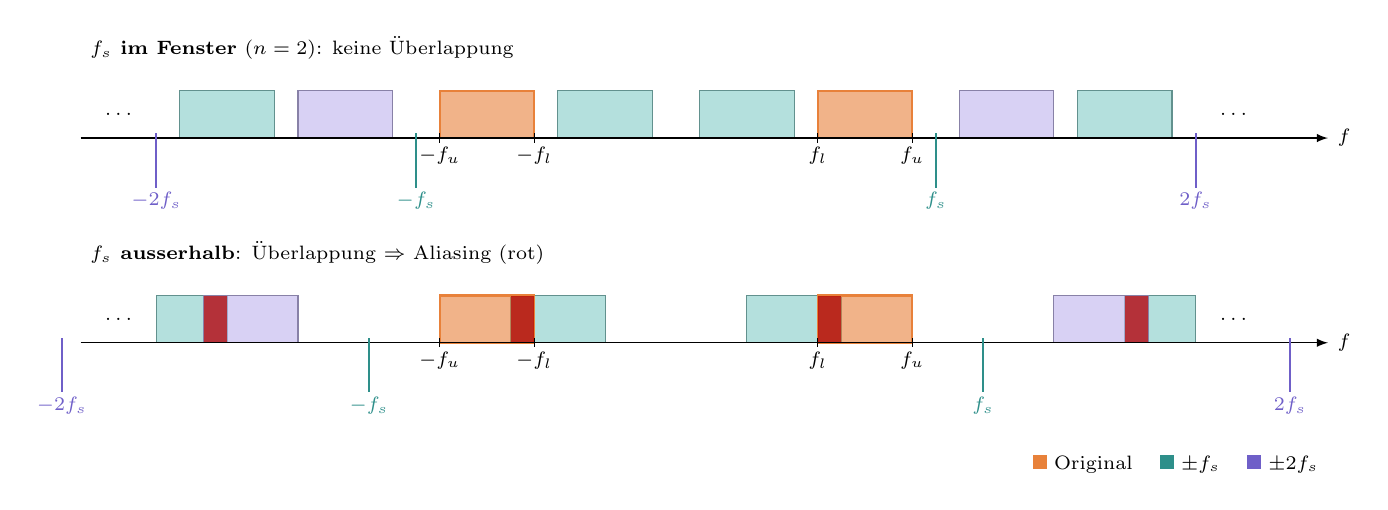
\begin{tikzpicture}[x=0.6cm,y=0.6cm,lab/.style={font=\scriptsize}]
\definecolor{org}{HTML}{E8813A}
\definecolor{kA}{HTML}{8CCFCB}\definecolor{kAd}{HTML}{2E8F8A}
\definecolor{kB}{HTML}{C3B8EE}\definecolor{kBd}{HTML}{6F5FC8}
\def\kopie#1#2#3{\fill[#3,fill opacity=0.65,draw=#3!70!black,thin] (#1,0) rectangle (#2,1);}
\def\orig#1#2{\fill[org,fill opacity=0.6,draw=org,thick] (#1,0) rectangle (#2,1);}
\def\ueber#1#2{\fill[red!70!black,fill opacity=0.75] (#1,0) rectangle (#2,1);}
\def\achse{\draw[-latex] (-12.6,0) -- (13.8,0) node[lab,right] {$f$};
  \foreach \x/\t in {-5/-f_u,-3/-f_l,3/f_l,5/f_u} \draw (\x,0.1) -- (\x,-0.1) node[lab,below,yshift=2pt] {$\t$};
  \node[lab] at (-11.8,0.5) {$\ldots$}; \node[lab] at (11.8,0.5) {$\ldots$};}
\def\ftick#1#2#3{\draw[#2,thick] (#1,0.1) -- (#1,-1.05) node[lab,below,text=#2,yshift=2pt] {$#3$};}
% Zeile 1: f_s im Fenster (f_s = 5,5)
\node[lab,anchor=west] at (-12.6,1.9) {\textbf{$f_s$ im Fenster} ($n=2$): keine Überlappung};
\kopie{0.5}{2.5}{kA} \kopie{8.5}{10.5}{kA} \kopie{-2.5}{-0.5}{kA} \kopie{-10.5}{-8.5}{kA}
\kopie{6}{8}{kB} \kopie{-8}{-6}{kB}
\orig{3}{5} \orig{-5}{-3}
\achse
\ftick{5.5}{kAd}{f_s} \ftick{-5.5}{kAd}{-f_s} \ftick{11}{kBd}{2f_s} \ftick{-11}{kBd}{-2f_s}
% Zeile 2: f_s ausserhalb (f_s = 6,5)
\begin{scope}[yshift=-2.6cm]
\node[lab,anchor=west] at (-12.6,1.9) {\textbf{$f_s$ ausserhalb}: Überlappung $\Rightarrow$ Aliasing (rot)};
\kopie{1.5}{3.5}{kA} \kopie{9.5}{11}{kA} \kopie{-3.5}{-1.5}{kA} \kopie{-11}{-9.5}{kA}
\kopie{8}{10}{kB} \kopie{-10}{-8}{kB}
\orig{3}{5} \orig{-5}{-3}
\ueber{3}{3.5} \ueber{-3.5}{-3} \ueber{9.5}{10} \ueber{-10}{-9.5}
\achse
\ftick{6.5}{kAd}{f_s} \ftick{-6.5}{kAd}{-f_s} \ftick{13}{kBd}{2f_s} \ftick{-13}{kBd}{-2f_s}
\end{scope}
\node[lab,anchor=east] at (13.8,-6.9) {\textcolor{org}{\rule{5pt}{5pt}} Original \;\; \textcolor{kAd}{\rule{5pt}{5pt}} $\pm f_s$ \;\; \textcolor{kBd}{\rule{5pt}{5pt}} $\pm 2f_s$};
\end{tikzpicture}}
\end{center}

{\small \textbf{Warum?} Kopie $n-1$ des Spiegelbands endet vor $f_l$ $\Rightarrow$ $f_s \le \frac{2 f_l}{n-1}$; Kopie $n$ beginnt nach $f_u$ $\Rightarrow$ $f_s \ge \frac{2 f_u}{n}$}\\[.4em]
\definecolor{ardesia}{HTML}{4A4D52}\definecolor{papier}{HTML}{F6F5F1}
\efbox[linecolor=ardesia,backgroundcolor=papier]{\begin{minipage}{.96\linewidth}
\textbf{Rezept}\\[.1em]
{\renewcommand{\arraystretch}{1.4}
\begin{tabularx}{\linewidth}{l X}
	1. & $B = f_u - f_l$, \quad $n_{sub} = \left\lfloor \dfrac{f_u}{B} \right\rfloor$ \\
	2. & \textbf{für jedes} $n = 1, 2, \ldots, n_{sub}$: \; \efbox[linecolor=red]{$\dfrac{2 f_u}{n} < f_s < \dfrac{2 f_l}{n-1}$} \quad ($n=1$: nur $f_s > 2 f_u$) \\
	3. & $f_s$ in einem Fenster $\Rightarrow$ kein Aliasing, sonst Aliasing. \quad $f_{s,min} \approx \dfrac{2 f_u}{n_{sub}}$ \\
\end{tabularx}}
\end{minipage}}\\[.3em]
{\small \textrightarrow\ zwischen den Fenstern liegt Aliasing: nicht jedes $f_s \ge f_{s,min}$ geht! Rückgewinnung mit \textbf{Bandpass}}\\
{\small \textrightarrow\ Folien: strikte Ungleichungen (bei Gleichheit schliesst sich das Fenster; ist $f_u/B$ ganzzahlig, dann $n_{sub} = \frac{f_u}{B} - 1$)}
\paragraph{Interpolation im digitalen Bereich S. 92 (Oversampling)}
Bei Oversampling werden auf \textbf{digitaler Seite Zwischenwerte berechnet} (Interpolation) um mehr Samples zu generieren vor der D/A Wandlung. Das führt dazu, dass das \textbf{Basisband erweitert} wird (also die Blöcke im Amplitudendichtespektrum auseinandergeschoben werden, vgl Abbildung unten und "ideale Abtastung").\\
\vspace{.3cm}
Berechnung der Zwischenwerte: \efbox[linecolor=red]{$m(t)=\sum_{n=-\infty}^{\infty} m(nT_0) \frac{sin(\omega_c(t-nT_0))}{\omega_c(t-nT_0)} \text{  mit  } \omega_c = \frac{\omega_s}{2}$}\\
\textbf{Vorteile:} TP-Filter kann einfacher realisiert werden (\textbf{weniger Steilheit} erforderlich), Signal wird originalgetreuer rekonstruiert; Amplitudengang des ZOH kann digital kompensiert werden.\\
{\small \textrightarrow\ $n$-fache Interpolation: analoges Filter mit Durchlass $0\ldots f_s/2$ sperrt erst ab $\left(n - \tfrac{1}{2}\right) \cdot f_s$}

\begin{center}
	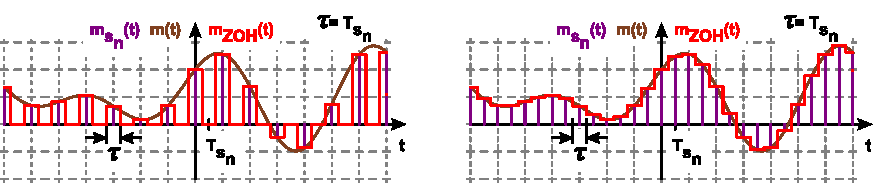
\includegraphics[width=.75\linewidth]{chapters/07_digsig/figures/abbildung6_6.pdf}\\
	Zweifach interpoliertes Zero-Order Hold Signal, vor und nach dem digitalen Tiefpassfilter\\
	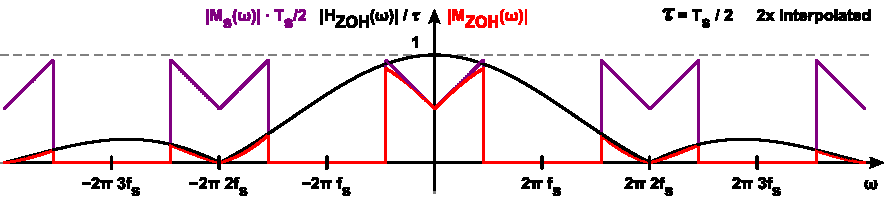
\includegraphics[width=.75\linewidth]{chapters/07_digsig/figures/abbildung6_7.pdf}\\
	Zweifach interpoliertes Zero-Order Hold Signal im Frequenzbereich
\end{center}

\subsection{Quantisierung S. 93}
Nach dem Sampling liegen die zeitdiskreten Abtastwerte noch immer \textbf{amplitudenkontinuierlich} vor!
\subsubsection{Gleichförmige Quantisierung S.93}

\begin{tabularx}{\linewidth}{p{.25\linewidth} p{.2\linewidth} p{.25\linewidth} p{.2\linewidth}}
	Skalierung von $m(t)$:    & $|m_n(t)| \le 1$ & Wortlänge der Samples: & n Bits \\
	Quantisierungsintervalle: & $L = 2^n$     & Intervallbreite:       & $\Delta = 2/L = 2^{-(n-1)}$
\end{tabularx}\\

\paragraph{Quantisierungsrauschen}
\begin{tabularx}{\linewidth}{p{.3\textwidth} p{.65\textwidth}}
	Fehlersignal $q_e(nT)$:	& Abweichung vom effektiven Wert zum quantisierten Wert. Char. von weissem Rauschen $->$ gleichverteilt im Intervall $-\Delta/2 ... \Delta/2$\\
	Maximaler Fehler:		&  $-\Delta/2 < q_e(nT_s) < \Delta/2$ \hspace{2cm} \efbox[linecolor=red]{$P_{qe}=N=\frac{1}{\Delta} \int_{-\Delta/2}^{\Delta/2} q_e^2dq_e = \frac{\Delta^2}{12}$}
\end{tabularx}\\
{\small \textrightarrow\ $m_d = m_s + q_e$; $q_e$ wirkt als weisses Rauschen nur bei $n \ge 8$ bit und stochastischem Signal}\\

\paragraph{SNR Signal-Rausch Verhältnis S. 93}
\begin{tabularx}{\linewidth}{p{.45\linewidth} p{.5\linewidth}}
	\begin{minipage}{\linewidth}
			\begin{list}{$\bullet$}{\setlength{\itemsep}{0cm} \setlength{\parsep}{0cm}
				\setlength{\topsep}{0cm}} 
			\item Signal wird maximal ausgesteuert mit\\ $|m(t)|_max = 1$
			\item $|m(t)|$ ist über Intervall $[-1...1]$ gleichverteilt
		\end{list}
	\end{minipage}
&
\begin{minipage}{\linewidth}
	\boxedeq{\begin{split} SNR_q=\frac{S}{N_q}=\frac{m^2_{RMS}}{\frac{\Delta^2}{12}} = \frac{P_m}{P_{qe}}= \frac{(\frac{1}{C})^2}{\frac{(\frac{1}{2^{n-1}})^2}{12}} = \frac{3}{C^2} \cdot 2^{2n} \\
	SNR_{q,dB} = n \cdot \qty{6.02}{\dB} + 10 \cdot log_{10} (\frac{3}{C^2}) \qty{ }{\dB} \end{split}}
\end{minipage}
\end{tabularx}\\
{\small \textrightarrow\ Sinus: $C = \sqrt{2} \Rightarrow +1.76$ dB \quad · \quad gleichverteilt: $C = \sqrt{3} \Rightarrow 0$ dB, also $SNR_q \approx n \cdot 6$ dB}

\subsubsection{Ungleichförmige Quantisierung S. 94}
	\begin{list}{$\bullet$}{\setlength{\itemsep}{0cm} \setlength{\parsep}{0cm}
		\setlength{\topsep}{0cm}} 
		\item Bei gleichförmiger Quantisierung ist N konstant $\rightarrow$ Verschlechterung der SNR bei tiefen Signalpegeln
		\item bei \textbf{Sprachsignalen vorwiegend kleine Pegel} (nicht gleichverteilt!)
		\item Quantisierungsintervalle $\Delta$ sind für kleine Signalpegel klein und für grosse Signalpegel grösser $\rightarrow$ SNR wird verbessert
	\end{list}

\paragraph{A-Law nach G.711 (diskret)}
$f_s = 8$ kHz $\cdot$ 8 bit = 1 Vorzeichen + 7 Amplitude $\cdot$ Band $300\ldots3400$ Hz; intern 12 bit linear\\
{\renewcommand{\arraystretch}{1.5}
\begin{tabular}{l l l l}
	\textbf{Bereich} & \textbf{$\Delta$} & \textbf{Intervalle} & \textbf{$\approx$ Auflösung} \\ \hline
	$0 \ldots \tfrac{1}{64}$ & $\tfrac{1}{2048}$ & 32 & 12 bit \\
	$\tfrac{1}{64} \ldots \tfrac{1}{32}$ & $\tfrac{1}{1024}$ & 16 & 11 bit \\
	$\ldots$ & $\Delta$ verdoppelt sich & je 16 & $-1$ bit pro Segment \\
	$\tfrac{1}{2} \ldots 1$ & $\tfrac{1}{32}$ & 16 & 6 bit \\
\end{tabular}}\\
{\small \textrightarrow\ $SNR \approx 40$ dB konstant für $\bar{S}/S_{max} \approx -36\ldots-6$ dB}\\
{\small \textrightarrow\ u-Law (USA): gleiche Kennwerte, andere Intervalle und Codes}

\subsection{Codierung}
{\renewcommand{\arraystretch}{1.4}
\begin{tabular}{l l}
	linear: & \texttt{0x0000}\ldots\texttt{0xFFFF} vom tiefsten zum höchsten Intervall \\
	Zweierkomplement: & positiv \texttt{0x0000}\ldots\texttt{0x7FFF}, negativ \texttt{0x8000}\ldots\texttt{0xFFFF} \\
\end{tabular}}\\
{\small \textrightarrow\ Zweierkomplement = linear mit invertiertem MSB}
\vfill

\subsection{Deltamodulator S. 99}
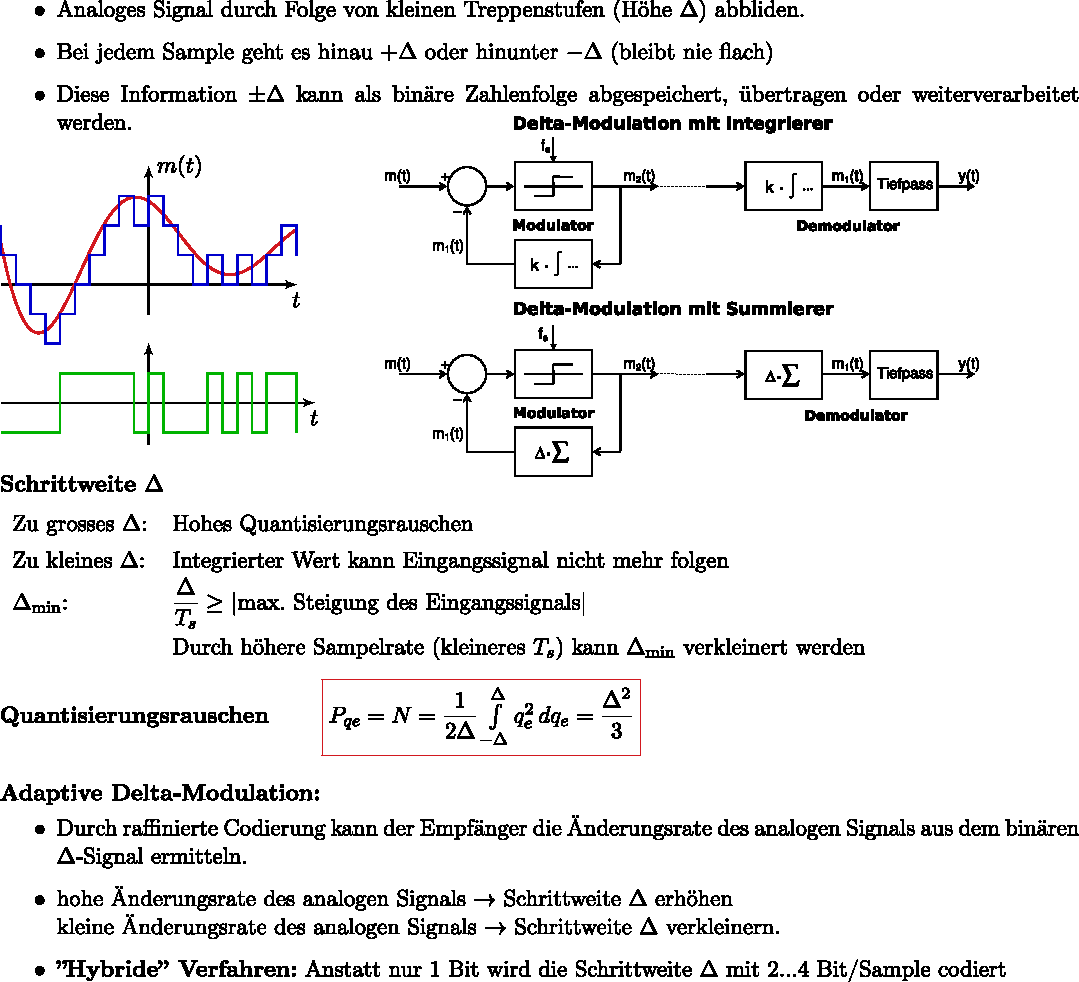
\includegraphics[width=.95\linewidth]{chapters/07_digsig/figures/deltamodulator.pdf}\\
\subsection{Delta-Sigma Modulator S. 100}
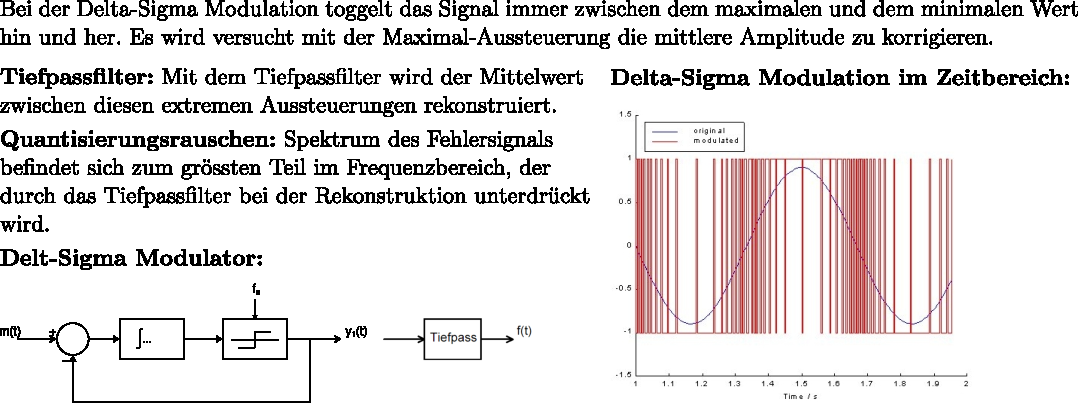
\includegraphics[width=.95\linewidth]{chapters/07_digsig/figures/deltasigmamodulator.pdf}\\
